\chapter{Atomic Mass and Chemical Reactions}


\section{Atomic and Molecular Mass}
%fixme add hook

\subsection{Reading a Periodic Tile}

Let us look at the different information shown on a periodic tile:

\begin{center}
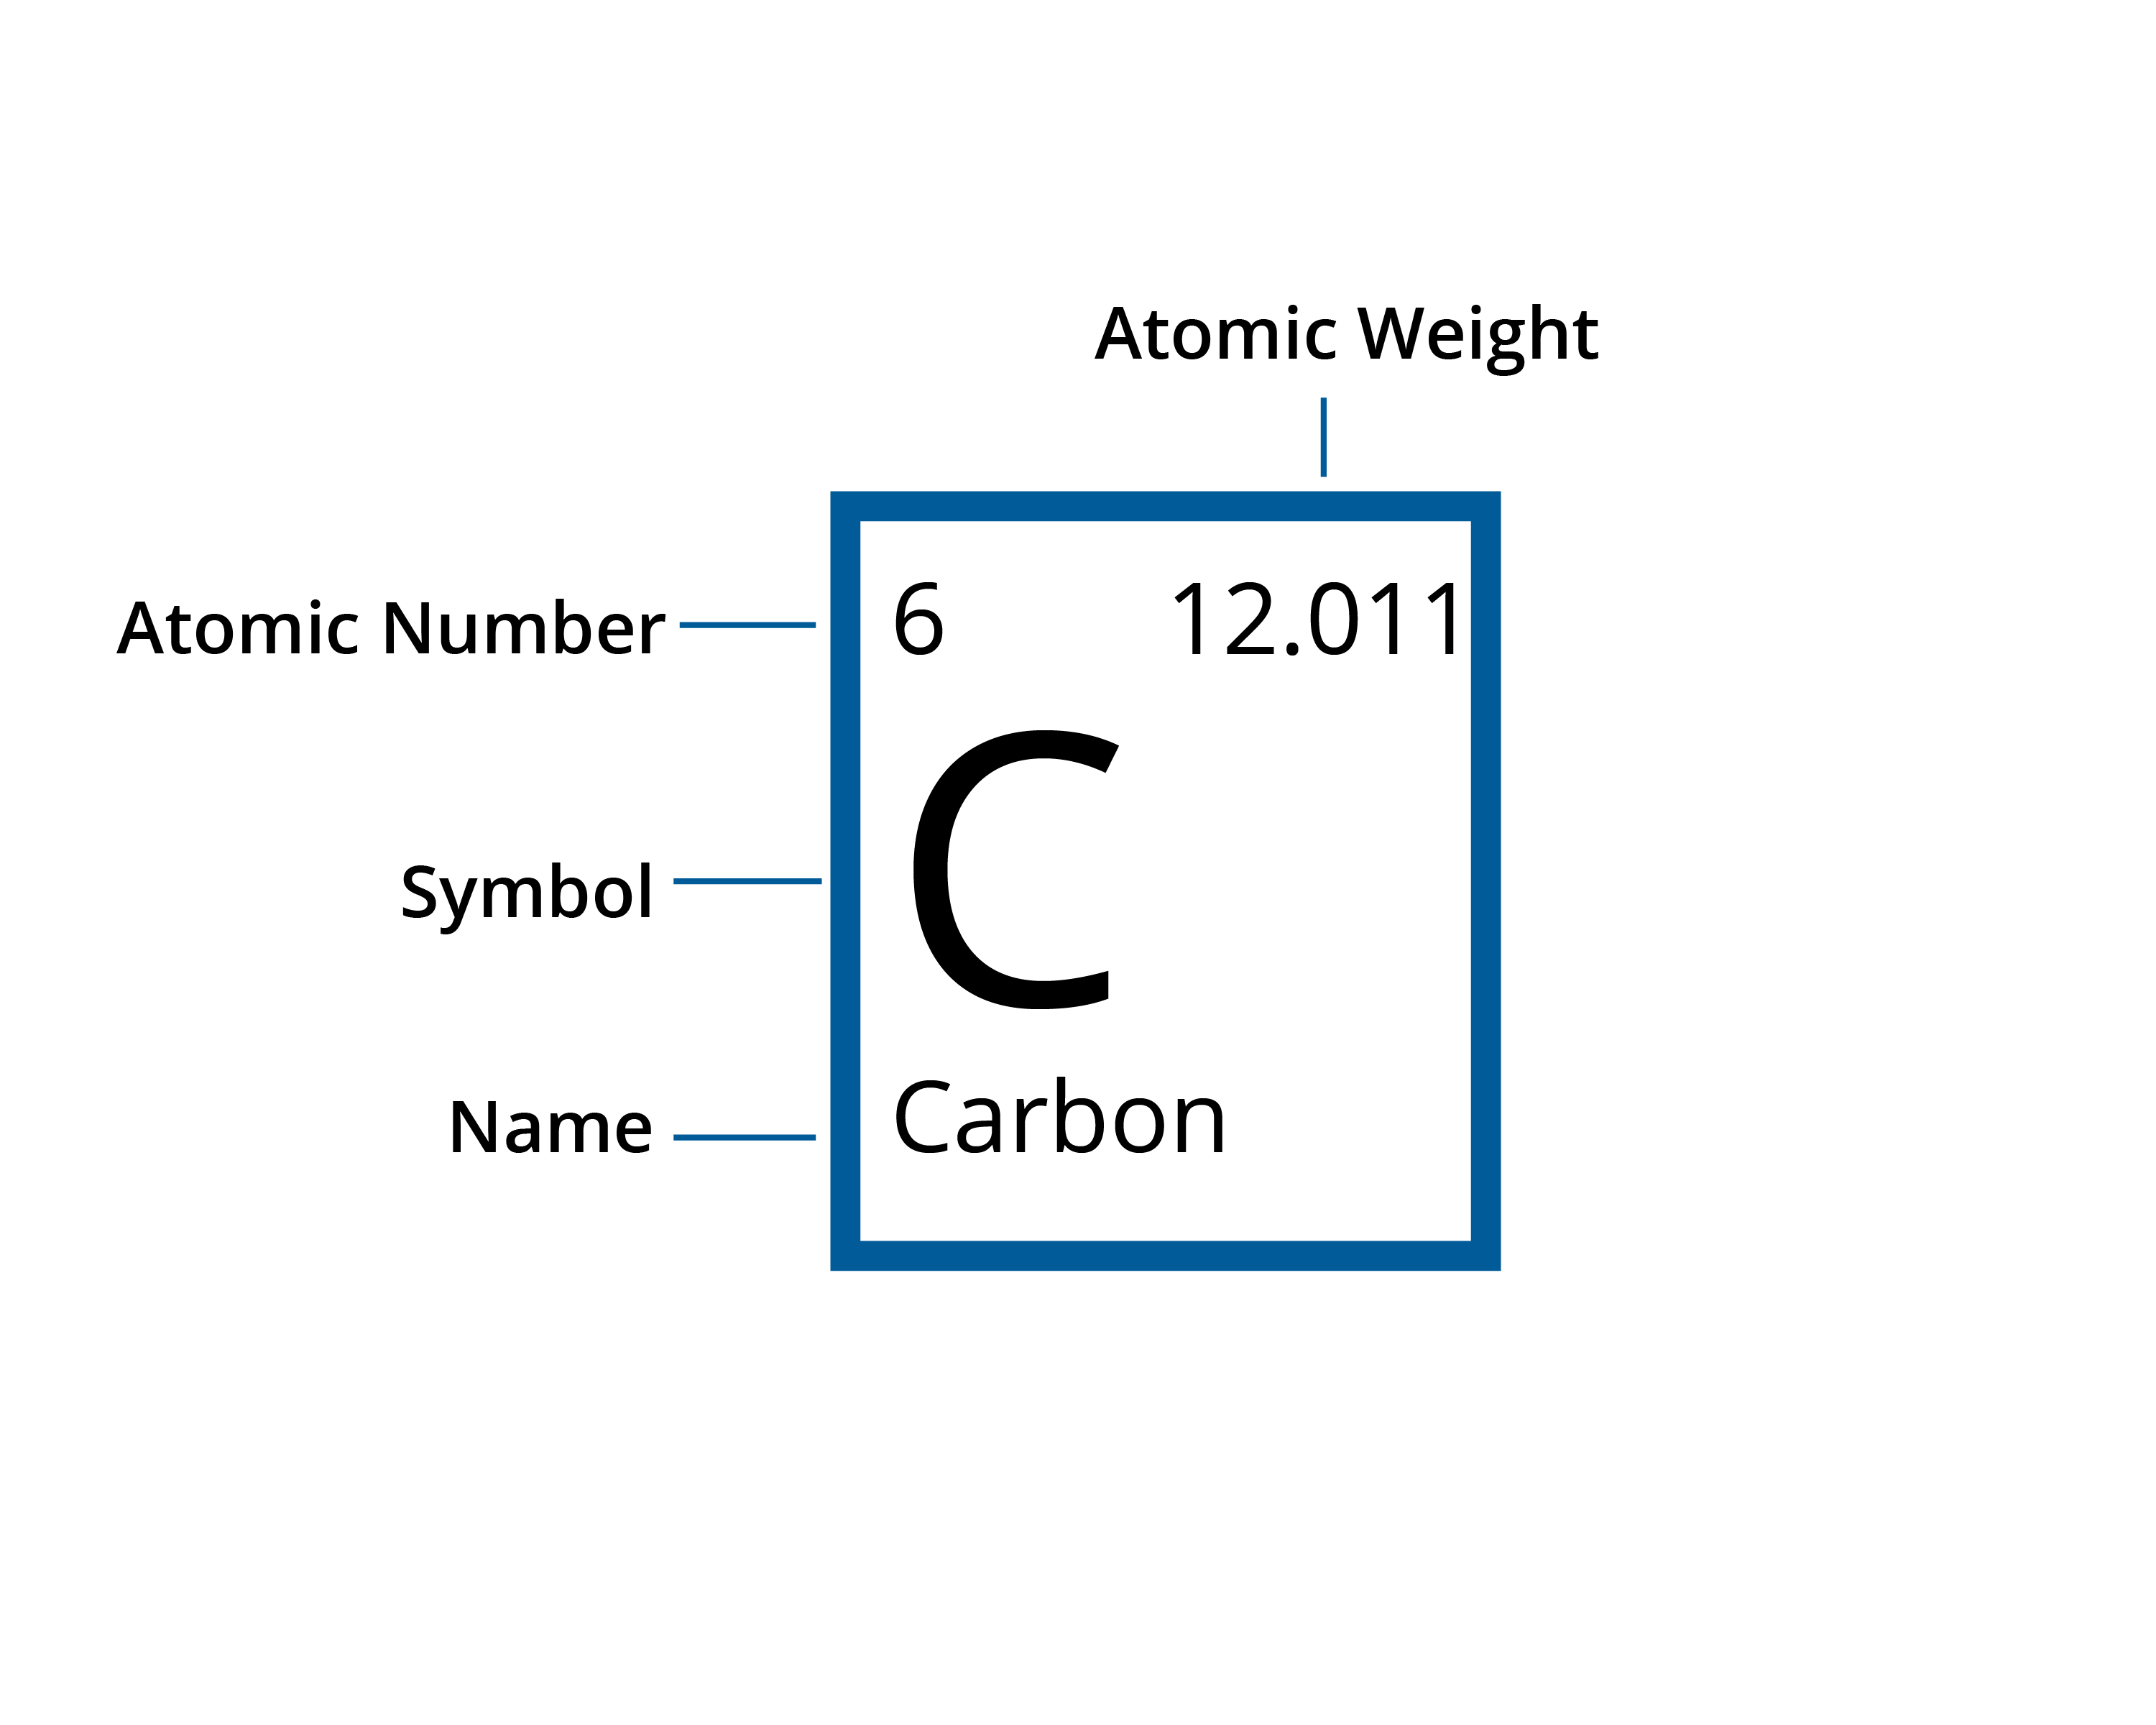
\includegraphics[width = 4in]{element.png}
%fixme change "weight" to "mass" or remake image
\end{center}

The four things we learn from a periodic tile are:
\begin{enumerate}
\item the symbol: as discussed in the previous chapter, each element has a 
unique symbol. Element symbols are used when showing the structure of a molecule
and modeling chemical reactions. 
\item the atomic number: this is also unique for each element. Take a look at the
periodic table a few pages forward. Every tile has a unique atomic number, and 
the tiles are laid out in a generally increasing atomic number (you will learn why
the periodic table is arranged this way in Sequence 2). 
\item the \index{atomic weight}atomic weight: this is the average mass of all the atoms of that element
in existence. Just like your overall grade in a class is the weighted average of
all the individual grades you earned, atomic weight is the weighted average of the
masses of all the individual atoms of that element. This is also sometimes referred to as atomic mass.
\item the name: not all periodic tables show the name of an element on its tile.
This is why it is useful to know the symbols of common elements. 
\end{enumerate}

Recall from the previous chapter that we classify atoms by the number of protons
they have. What this means is that if we want to know what element an atom is, we
have to look at the number of protons. Take a look at the three carbon atoms below
and note what is the same and what is different among them:

\begin{center}
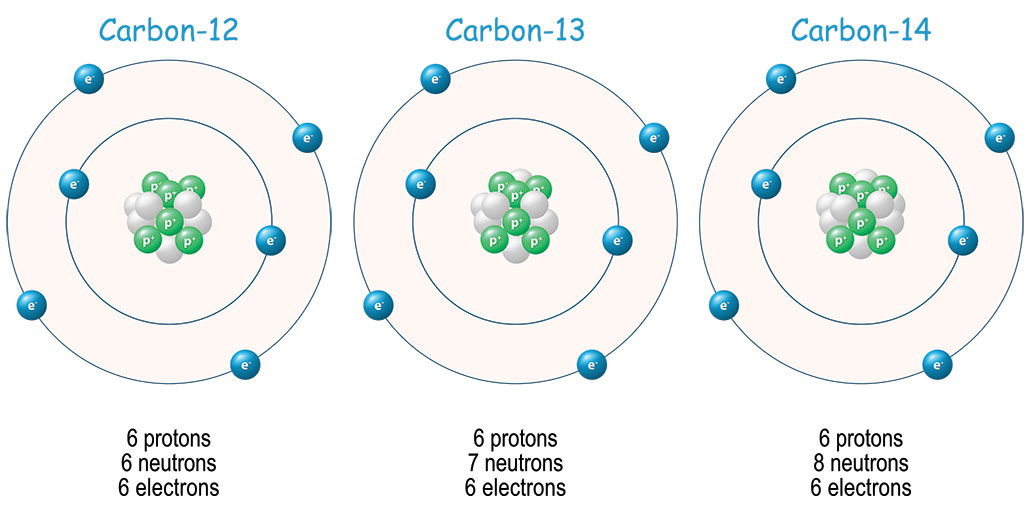
\includegraphics[scale=0.35]{carbon_iso.png}
\end{center}

These different versions of carbon all have 6 protons, which is also carbon's 
atomic number. This is not a coincidence: the \index{atomic number}atomic number \textit{is} the number
of protons in every atom of an element. If I tell you an atom has 4 protons, you 
would find atomic number 4 and see that the element is beryllium. To know how many
protons an oxygen atom has, you would find its tile and see that it has atomic 
number 8. 

So atoms of the same element have the same number of protons, and
that number is the element's atomic number. The difference between these
carbon atoms explains the other number on a periodic tile: the atomic mass. 

A proton and a neutron have about the same mass. An electron, on the other hand,
is tiny: it takes about 1,800 electrons to match the mass of one neutron. 
This means that the mass of any object comes mostly from the protons and neutrons
in the nucleus of its atoms. \index{proton} \index{neutron}

We know how many protons an atom has by what element it is, but how do we know the 
number of neutrons?

\subsection{Mass of Atoms and Molecules}
As you have seen, a periodic tile for an element tells us the average mass of an 
atom of that element in Daltons or amus (atomic mass units). The average mass of a
carbon atom is 12.011 amu, and the average mass of an iron atom is 55.845 amu. 
Using the periodic table, determining the average mass of an atom is 
straightforward. What about molecules?

Consider water: $H_2 O$. It is made of 2 hydrogen atoms, each with an average 
mass of 1.008 amu, and one oxygen atom, with an average mass of 15.999 amu. To 
find the mass of the molecule, called \index{molecular mass}\textit{molecular mass}, you simply add the 
masses of each of the atoms in the molecule. So, the molecular mass of water is 
1.008 amu + 1.008 amu + 15.999 amu = 18.015 amu. 

\begin{Exercise}[title = {Determining Molecular Mass}, label = molecular]
Find the molecular mass, in amu, of the following substances:
\begin{enumerate}
\item $CH_4$
\item $CuSO_4$
\item $C_6H_{12}O_6$
\end{enumerate}
\end{Exercise} 

\begin{Answer}[ref = molecular]
\begin{enumerate}
\item 12.011 amu + 4(1.008 amu) = 16.043 amu
\item 63.546 amu + 32.06 amu + 4(15.999 amu) = 159.602 amu
\item 6(12.011 amu) + 12(1.008 amu) + 6(15.999) amu = 180.156 amu
\end{enumerate}
\end{Answer}

\subsection{Mole Concept}

An atomic mass unit is a very, very, very small unit; we would much rather work in
grams. Grams are a large enough unit that you can develop a natural sense for how 
much a gram is. Additionally, while you cannot see a single carbon atom with your 
eyes, you can see 10 grams of carbon (about enough to fill a pen cap). To convert
between the very, very, very small unit of amus to the tangible unit of grams, we 
use \textit{Avogadro's Number} (sometimes called \textit{Avogadro's Constant}).
\index{Avogadro's number}

Since 1 amu is defined as $1/12^{th}$ of the mass of a carbon-12 atom, carbon-12 
by definition has a mass of 12 amu. Additionally, Avogadro's number is the number 
of carbon atoms in 12.000 grams of pure carbon-12. This amount is called \textit{a
mole}. A mole is just a counting word, like a dozen. Twelve doughnuts is a dozen doughnuts. Twenty is a score. Five hundred is a ream. And $6.02214076 
\times 10^{23}$ doughnuts is a \textit{mole} of doughnuts, enough to bury the entire Earth under a layer of doughnuts more than 100 km deep. That is why we save moles for tiny things like atoms and molecules.\index{mole} (A mole is not short for ``molecule''; the names just sound alike.) To get a feel for how huge this number is, watch this video: 
\url{https://www.youtube.com/watch?v=TEl4jeETVmg}. 
A mole of carbon-12 has a mass of 12.000 g, but a mole of natural carbon (which
includes all the isotopes of carbon) has a mass of 12.011 g. The mole is defined 
such that one mole of an element is the same mass in grams as one atom is in amus.
Let us say you want to know how much a mole of $NaCl$ weighs. From the periodic 
table, you see that $Na$ has an atomic mass of 22.990 atomic mass units, and $Cl$ 
has 35.453 atomic mass units. One unit of $NaCl$ (one sodium plus one chlorine) has a mass of $22.990 + 35.453 = 
58.443$ atomic mass units. This means a mole of $NaCl$ has a mass of $58.443$ 
grams. Handy, right? This is called the \index{molar mass}\textit{molar mass}. It is the mass of one
mole of a substance, and is given in units of $g/mol$ (grams per mole). The molar 
mass of NaCl is 58.443 g/mol. The molar mass of carbon is 12.011 g/mol. Using 
dimensional analysis and the molar mass, you can determine the mass of a given 
number of moles of a substance. 
% ADD: clarify here that g/mol is numerically equivalent to amus but conceptually different

\textbf{Example}: What is the mass of 2 moles of copper?

\textbf{Solution}: The conversion we will use is 1 mol Cu = 63.546 g Cu.
$$\frac{2 \text{ mol Cu}}{} \times \frac{63.546\text{ g Cu}}{1\text{ mol Cu}} = 
127.092\text{ g Cu}$$

Therefore, 2 moles of copper has a mass of 127.092 grams. 

You can also find the molar mass of a molecule, like methane. Just like with 
elements, a mole of a molecule has the same mass in grams as a single molecule has
in amus. 

\textbf{Example}: What is the mass of 3.5 moles of methane?

\textbf{Solution}: Methane ($CH_4$) has a molecular mass of 16.043 amu, which 
means 1 mole of methane has a mass of 16.043 grams. 

$$\frac{3.5\text{ mol }CH_4}{} \times \frac{16.043{ g }CH_4}{1\text{ mol }CH_4} = 
56.151\text{ g }CH_4$$

You can also use the molar mass to determine how many moles of a substance there 
are in a given mass of that substance.

\textbf{Example}: A standard AAA battery contains about 7.00 g of zinc. How many 
moles of zinc are in a AAA battery?

\textbf{Solution}: Zinc's molar mass is 65.38 g/mol. 
$$\frac{7.00\text{ g Zn}}{} \times \frac{1\text{ mol Zn}}{65.38\text{ g Zn}} 
\approx 0.107\text{ mol Zn}$$

In summary, a mole of a substance contains approximately $6.02 \times 10^{23}$ 
particles (atoms or molecules) of that substance and has a mass equal to the 
molecular mass in grams. 

\begin{mdframed}[frametitle = {The Mole Concept}, style = important]
For a substance, X, with a molar mass of $x$ g/mol,
$$1\text{ mol X } = 6.02 \times 10^{23}\text{ particles of X }= x\text{ g of X}$$
\end{mdframed}

\begin{Exercise}[title = {Grams, Moles, Molecules, and Atoms}, label = convert]
Complete the table.

\begin{tabular}{|c|c|c|c|}
\hline
Substance & num. of particles & num. of moles & grams\\\hline
$NaHCO_3$ & & & 35\\\hline
$HCl$ & & 1.25 & \\\hline
$KH_2PO_4$ & $12.5 \times 10^{24}$ & & \\\hline
\end{tabular}
\vspace{75mm}
\end{Exercise}

\begin{Answer}[ref = convert]
\begin{tabular}{|c|c|c|c|}
\hline
Substance & num. of particles & num. of moles & grams \\\hline
$NaHCO_3$ & $2.509 \times 10^{23}$ & 0.4166 & 35.00 \\\hline
$HCl$ & $7.53 \times 10^{23}$ & 1.25 & 45.58 \\\hline
$KH_2PO_4$ & $12.5 \times 10^{24}$ & 20.8 & 2820 \\\hline
\end{tabular}

$$\frac{35.00\text{ g }NaHCO_3}{} \times 
\frac{1\text{ mol } NaHCO_3}{84.007\text{ g }NaHCO_3} = 0.4166\text{ mol }NaHCO_3$$

$$\frac{0.4166\text{ mol }NaHCO_3}{} \times \frac{6.02214076 
\times 10^{23}\text{ molec }NaHCO_3}{1\text{ mol }NaHCO_3} = 
2.509 \times 10^{23}\text{ molec }NaHCO_3$$

$$\frac{1.25\text{ mol }HCl}{} \times 
\frac{36.46\text{ g }HCl}{1\text{ mol }HCl} = 45.58\text{ g }HCl$$

$$\frac{1.25\text{ mol }HCl}{} \times 
\frac{6.02214076 \times 10^{23}\text{ molec }HCl}{1\text{ mol }HCl} 
= 7.53 \times 10^{23}\text{ molec }HCl$$

$$\frac{12.5 \times 10^{24}\text{ molec }KH_2PO_4}{} \times 
\frac{1\text{ mol }KH_2PO_4}{6.02214076 \times 10^{23}\text{ molec }KH_2PO_4} 
= 20.8\text{ mol }KH_2PO_4$$

$$\frac{20.8\text{ mol }KH_2PO_4}{} \times 
\frac{136.086\text{ g }KH_2PO_4}{1\text{ mol }KH_2PO_4} = 
2820\text{ g }KH_2PO_4$$
\end{Answer}

% ADD: Conversions should probably come before this

\begin{Exercise}[title={Burning Methane}, label=burning_methane]

Natural gas is mostly methane ($CH_4$). When one molecule of methane
burns, it uses up two oxygen molecules ($O_2$) and makes one molecule of
$CO_2$ and two molecules of $H_2O$:
$$CH_4 + 2O_2 \rightarrow CO_2 + 2H_2O$$
% ADD: Need to explain mole to mole ratios first, Law of Divine Proportion
% ADD: Include Significant Figures

If you need 200 grams of water, how many grams of methane do you need
to burn?

(The hero of \emph{The Martian} makes water for his potato farm in a similar way, by burning hydrogen.)
\vspace{50mm}
\end{Exercise}

\begin{Answer}[ref=burning_methane]

One mole of water has a mass of about 18.015 grams, so 200 grams of water is about $200 / 18.015 \approx 11.1$ moles. Each methane molecule makes \emph{two} water molecules, so you need half as many moles of methane: about 5.55 moles.

One mole of methane has a mass of $12.011 + 4 \times 1.008 = 16.043$ grams.

$16.043 \times 5.55 \approx 89.0$ grams of methane.

\end{Answer}


%final above, pieces below
If you fill a balloon with helium, it will have two different
kinds of helium atoms. Most of the helium atoms will have 2 neutrons, but a
few will have only 1 neutron. We say that these are two different
\textit{isotopes} of helium. We call them helium-4 (or $^4He$) and
helium-3 (or $^3He$). Isotopes are named for the sum of protons and
neutrons the atom has: helium-3 has 2 protons and 1 neutron.\index{isotopes}

A hydrogen atom nearly always has just 1 proton and no neutrons. A
helium atom nearly always has 2 protons and 2 neutrons. So, if you
have 100 hydrogen atoms and 100 helium atoms, the helium will have
about 4 times more mass than the hydrogen. We say ``Hydrogen is about
1 atomic mass unit (amu), and helium-4 is about 4 atomic mass
units.''\index{atomic mass unit}

What, precisely, is an atomic mass unit? It is defined as 1/12 of
the mass of a carbon-12 atom. Scientists have measured the mass of
helium-4, and it is about 4.0026 atomic mass units. (By the way, an
atomic mass unit is also called a \index{dalton}\textit{dalton}.)

\pagebreak


Now you are ready to take a good look at the periodic table of
elements. Here is the version from Wikipedia:\index{periodic table of elements}
\begin{figure}[H]
    \centering
    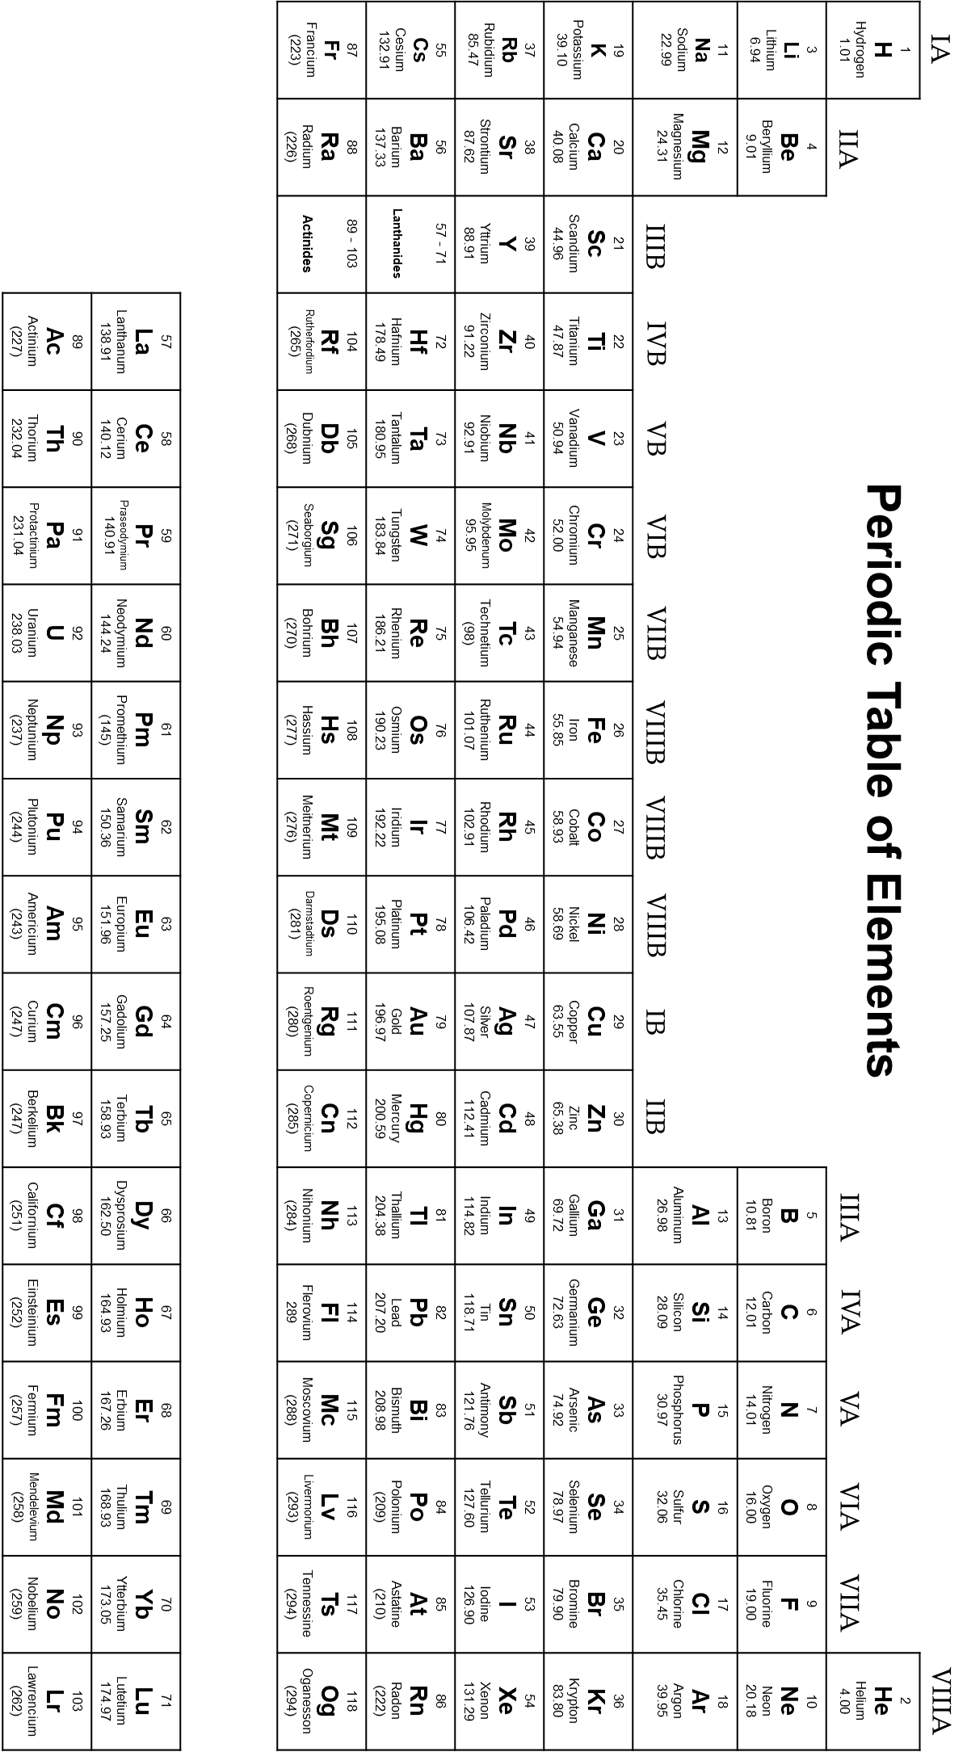
\includegraphics[width=0.75\textwidth]{periodic.png}
    \caption{Periodic table from Wikipedia.}
    \label{fig:periodic_tbl}
\end{figure}

% ADD: Periodic Trends, Periods, Columns, Atomic Radius, Electronegativity,

\pagebreak
There is a square for each element. In the middle, you can see the atomic
symbol and the name of the element. In the upper-right corner is the
atomic number --- the number of protons in the atom.

In the upper-left corner is the atomic mass in atomic mass units.\index{atomic mass}

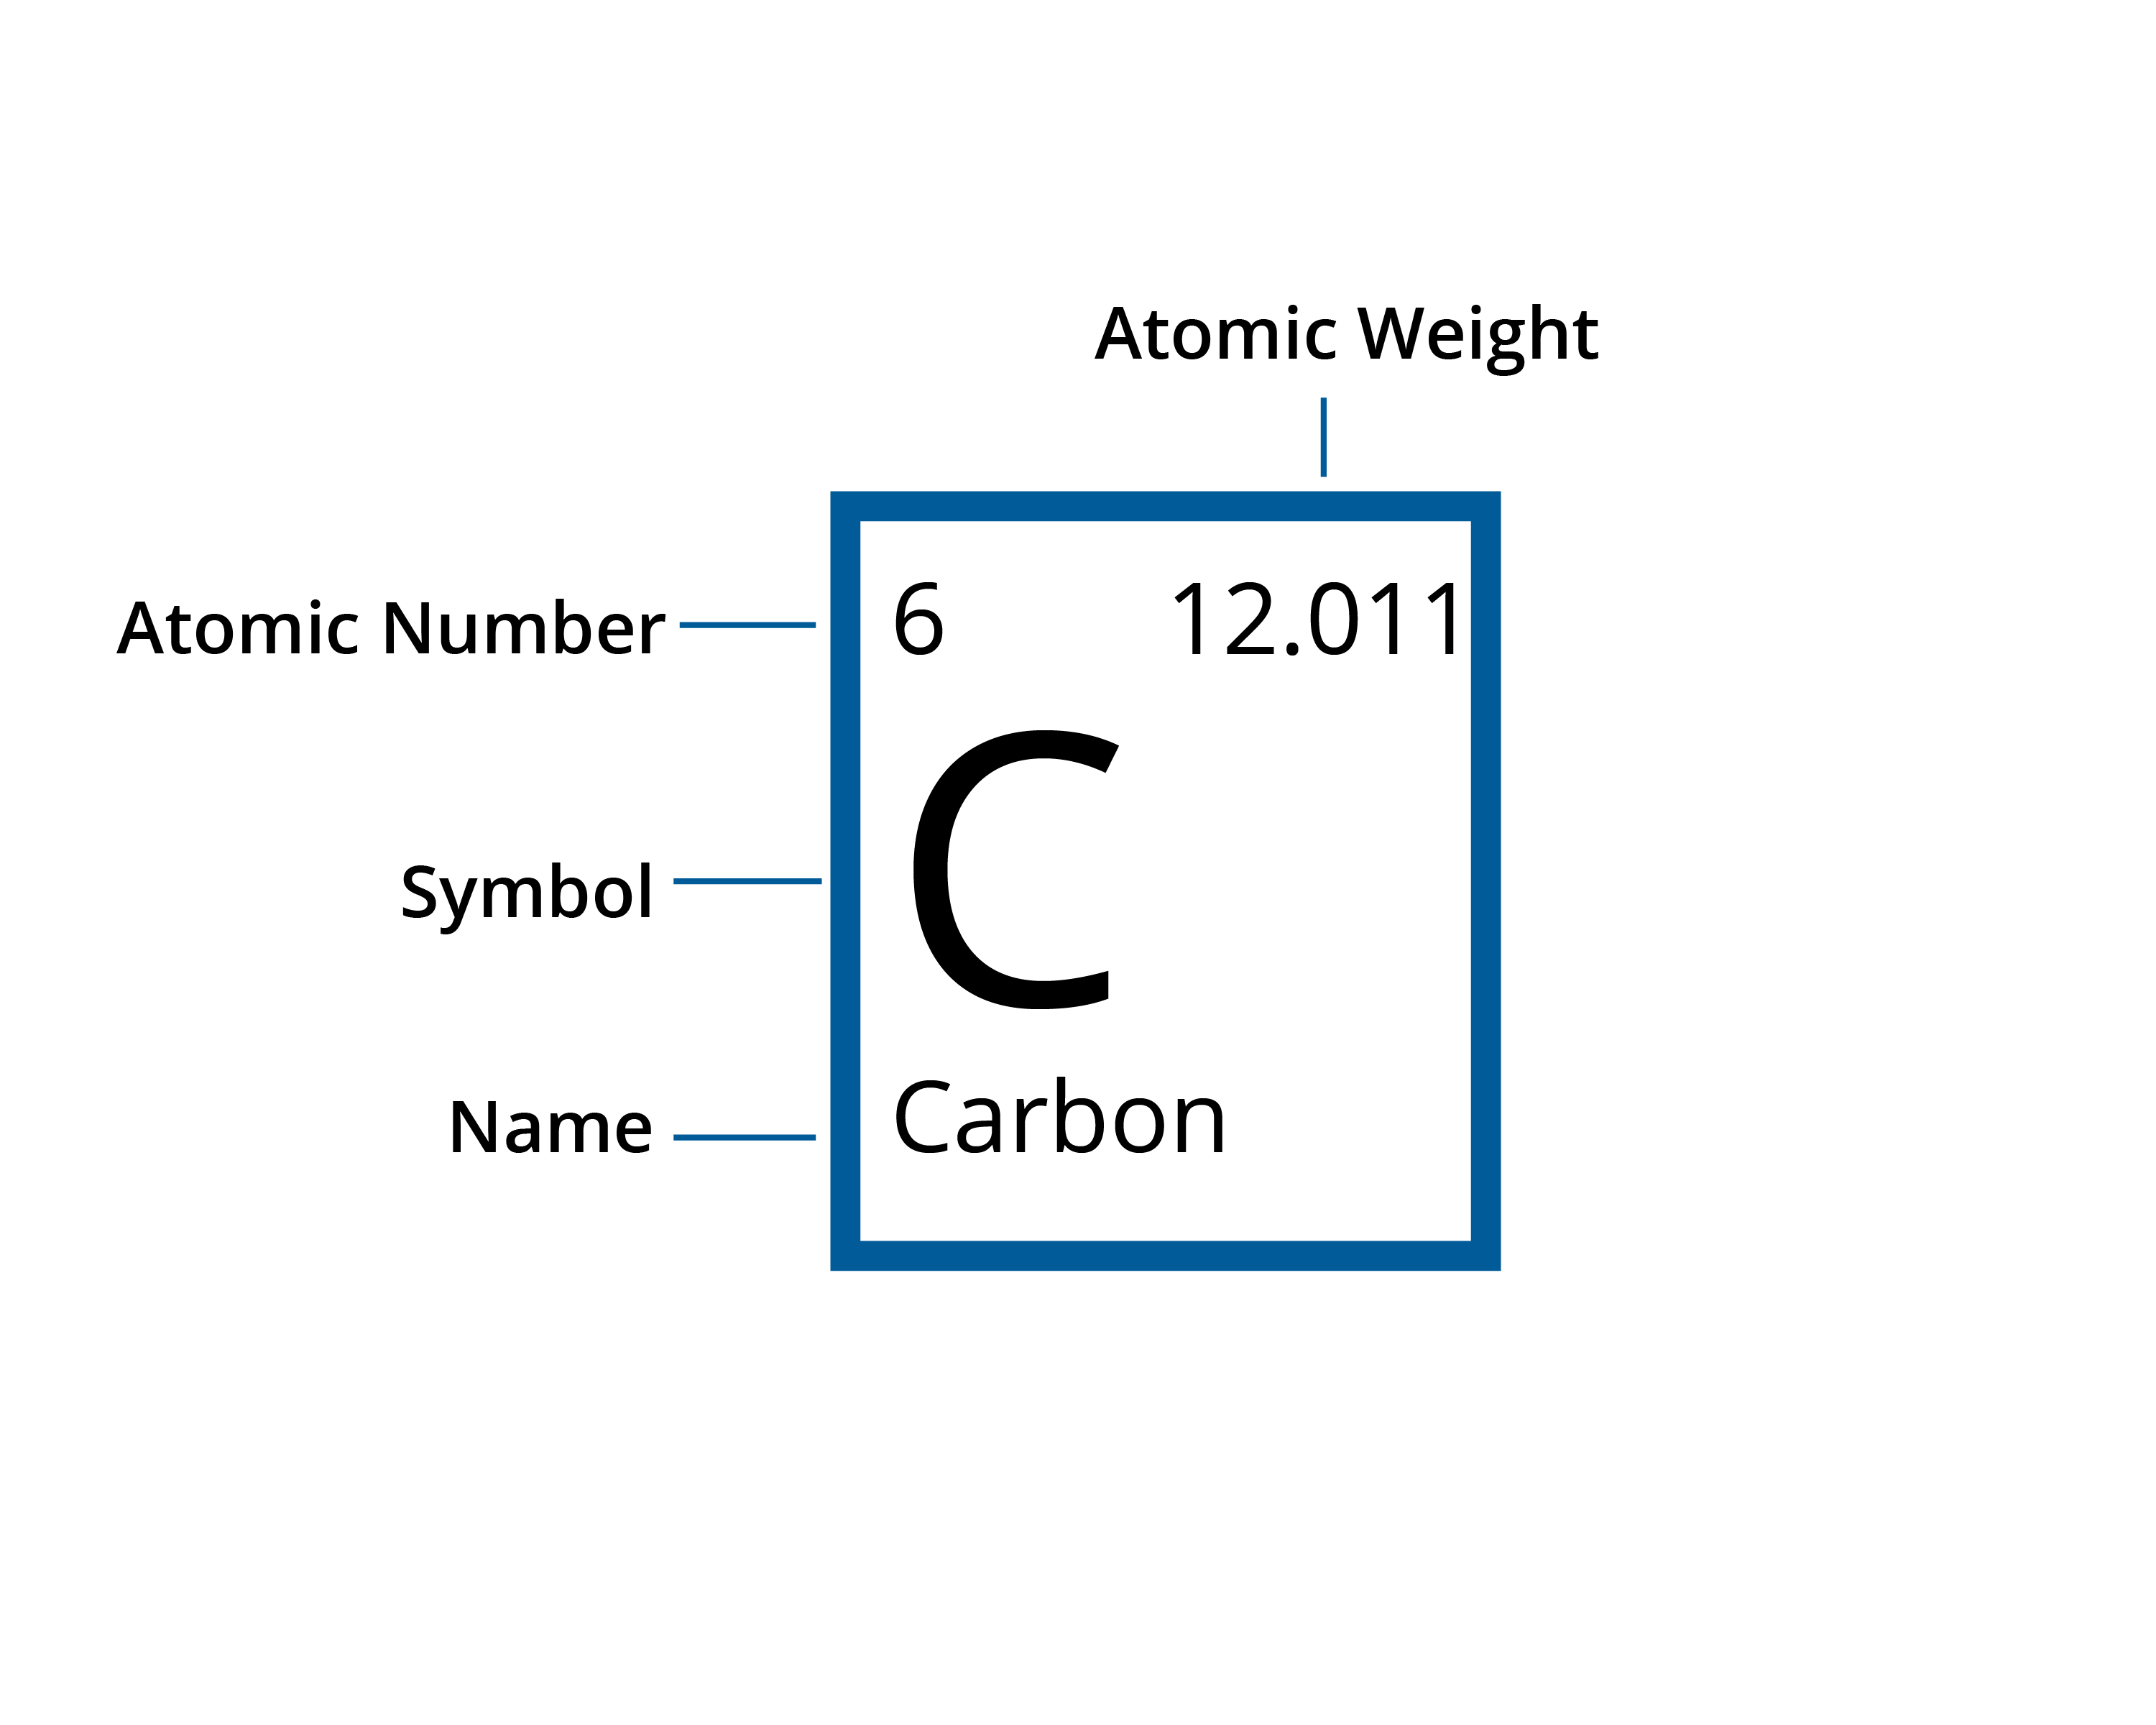
\includegraphics[width=0.8\textwidth]{element.png}

Look at the atomic mass of boron. About 80\% of all boron atoms have
six neutrons. The other 20\% have only 5 neutrons. This difference is why most boron atoms
have a mass of about 11 atomic mass units, but some have a mass of
about 10 atomic mass units. The atomic mass of boron is equivalent to the average
mass of a boron atom: 10.811.
% ADD: Talk about mass spectroscopy
%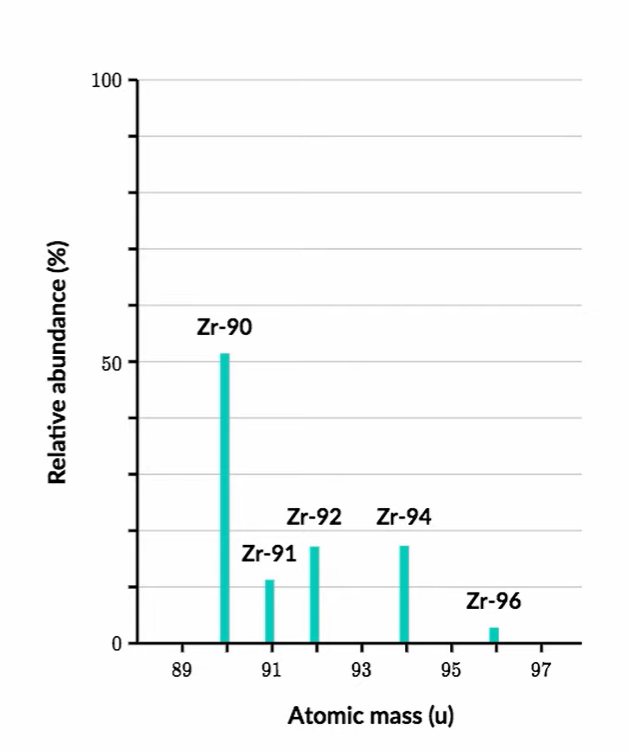
\includegraphics[width=0.75\textwidth]{KA_Mass_Spectroscopy_Zr.png}

\begin{Exercise}[title={Mass of a Water Molecule}, label=water_mass]

Using the periodic table, what is the average mass of one water molecule in atomic mass units?

\end{Exercise}
\begin{Answer}[ref=water_mass]

  The average hydrogen atom has a mass of 1.00794 atomic mass units.

  The average oxygen atom has a mass of 15.9994.

  $2 \times 1.00794 + 15.9994 = 18.01528$ atomic mass units.

\end{Answer}

\subsection{Reading the Periodic Table}
The Periodic Table organizes what we know about the structure of different
elements. Each element has its own block or tile on the Periodic Table, and the
information on the tile tells us about the structure of that atom. Take a look at
the tile for carbon:

\begin{center}
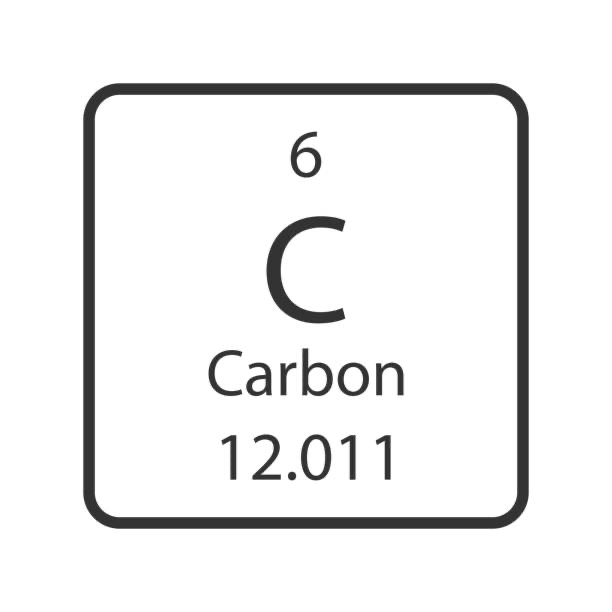
\includegraphics[width=2in]{carbon_tile.png}
\end{center}

The letter (or letters, as is the case for other elements) is the atomic symbol
for the element. There are two key numbers: the atomic number and the average
atomic mass. For carbon, the atomic number is 6 and the average atomic mass is
12.011. The atomic number tells us how many protons there are in the nucleus of
any atom of carbon. Since every element has a unique number of protons, every
element has a unique atomic number. All carbon atoms have 6 protons. The other
number is the average atomic mass - it tells us the weighted average of the
mass of all the carbons in the universe. When the average atomic mass is in
a whole number, as it is for polonium, it means that the element is very unstable.
As a result, the mass given is the mass of the most stable isotope (we will talk
more about stability and isotopes below). On some periodic tables, the mass
number of the most stable isotope will be in parentheses or brackets. In
summary, if the larger number is a whole number, it is the mass number; if it
is a decimal (even if the decimal ends in .00), it is the average atomic mass,
which we will discuss further below.

\begin{center}
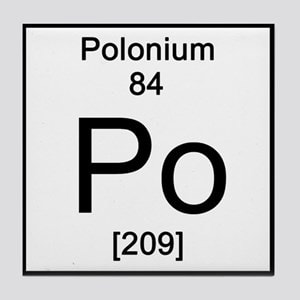
\includegraphics[width=2in]{polonium_tile.png}
\end{center}

The Royal Society of Chemistry has a very useful interactive periodic table:
periodic-table.rsc.org. We can use the periodic tile for an element to
determine the number of protons, electrons, and most common number of neutrons
for a neutral atom of that element (we will explain why the periodic tile tells
us the "most common number of neutrons" below).

\textbf{Example}: State the atomic symbol for and the number of protons,
neutrons, and electrons in a neutral atom of plutonium.

\textbf{Solution}: The plutonium tile on your periodic table should look
something like this:
\begin{center}
   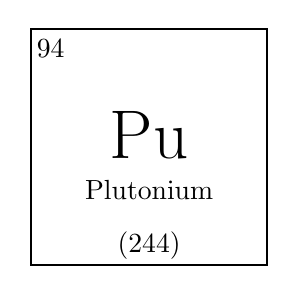
\begin{tikzpicture}
        \draw[black, thick] (-1.5, -1.5) rectangle (1.5,1.5);
        \node[font = \Huge] at (0,0.15) {Pu};
        \node[] at (-1.25, 1.25) {$94$};
        \node[] at (0, -0.55) {Plutonium};
        \node[] at (0, -1.25) {$(244)$};
    \end{tikzpicture}
\end{center}

[The information may be arranged differently, but you should at least see the
symbol and two numbers.] As you can see, the atomic symbol for plutonium is Pu.
Since its atomic number is 94, we know every atom of plutonium has 94 protons.
To know the number of electrons, we will take advantage of the fact that the
question is asking about a \textit{neutral} atom. This means there are the same
number of positive charges as negative charges. So, since there are 94 protons,
a neutral atom of plutonium must have 94 electrons (each proton has a +1 charge
and each electron has a -1 charge). Lastly, let us determine the number of
neutrons. The other number, 244, is the \index{mass number}mass number. It represents the total
number of protons and neutrons in the nucleus. Since we know plutonium has 94
protons, we can find the number of neutrons by subtracting the atomic number
from the mass number:

\begin{center}
   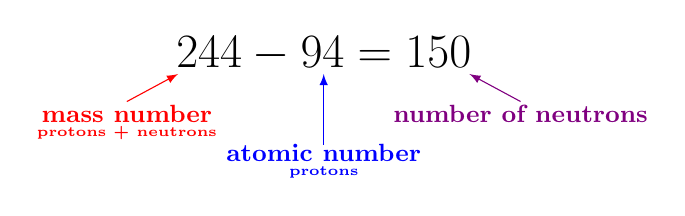
\begin{tikzpicture}
        \node[font = \LARGE] at (0,0) {$244 - 94 = 150$};
        \node[font = \small, red] at (-2.5, -0.75) {\textbf{mass number}};
        \node[font = \tiny, red] at (-2.5, -1) {\textbf{protons + neutrons}};
        \draw[red, -latex] (-2.5, -0.6) -- (-1.85, -0.25);
        \node[font = \small, blue] at (0, -1.25) {\textbf{atomic number}};
        \node[font = \tiny, blue] at (0, -1.5) {\textbf{protons}};
        \draw[blue, -latex] (0, -1.15) -- (0, -0.25);
        \node[font = \small, violet] at (2.5, -0.75) {\textbf{number of neutrons}};
        \draw[violet, -latex] (2.5, -0.6) -- (1.85, -0.25);
    \end{tikzpicture}
\end{center}

Therefore, an atom of plutonium has 150 neutrons. Now let us address how to find
the number of neutrons when the periodic tile shows an average atomic mass,
instead of a mass number. Plutonium has no stable ``versions'' and barely exists in nature, so there is no natural average to report; its tile shows the mass number of its longest-lived version, Pu-244. Most elements are different: they come in a natural mix of versions, and the tile shows the average mass. Carbon is a good example.

Have you heard of carbon-14 dating? The phrase "carbon-14" refers to a rare
type of carbon that decays radioactively. By seeing how much carbon-14 has
decayed, scientists can estimate the age of organic materials, such as bone or
ash. Carbon-14 is a radioactive isotope (or version) of carbon. The 14 refers to
the mass number - the total amount of protons and neutrons in the nucleus
(sometimes, we shorten the isotope name by just using the atomic symbol, in
this case C-14). Isotopes are versions of an element with different numbers of
neutrons. The atomic number is the same for them all - they all have the same
number of protons. But the different number of neutrons causes different
isotopes to have different masses. Examine the models of carbon-12, carbon-13,
and carbon-14 below. What is different between them? What is the same?



You should have noticed that all three atoms have 6 protons and 6 electrons,
while they have differing numbers of neutrons. The most common isotope of carbon
is carbon-12, with 6 protons and 6 neutrons in its nucleus. Carbon-14, on the
other hand, has 8 neutrons, which makes the nucleus unstable, leading to
radioactive decay. \index{average atomic mass}The average atomic mass
is the weighted average of all the carbon atoms in existence. Since the vast
majority of carbon is carbon-12, the average atomic mass is very close to 12.
You cannot determine the mass number of an individual atom from the periodic
table; it only tells you the average of all the isotopes. However, especially
for light atoms (atoms in the first two rows of the periodic table), you can
usually determine the mass number of the most common isotope by rounding the
average atomic mass to the nearest whole number.

\textbf{Example}: Sodium has atomic symbol Na. State the number of protons,
number of electrons, and most common number of neutrons in a neutral atom of
sodium.

\textbf{Solution}: Sodium's atomic number is 11, so a neutral atom has 11 protons and
11 electrons. The average atomic mass is 22.990, which rounds to 23. So the
most common isotope of sodium is Na-23, which has $23 - 11 = 12$ neutrons.

Be careful with heavier elements. Germanium's average mass is 72.630, which rounds to 73, but its most common isotope is actually Ge-74. When an element has several common isotopes, the average can land between them.

\begin{Exercise}[title = {Determining Numbers of Subatomic Particles}, label = pne]
Use a periodic table to complete the table below (assume neutral atoms): %fixme wrap text for neutrons column

\begin{tabular}{|c|c|c|c|c|}
\hline\\
Element Name & Atomic Symbol & Protons & Most Common Number of Neutrons & Electrons\\\hline
 & Fr & & & \\\hline
 & & & & 33\\\hline
 Aluminum & & & & \\\hline
  & & 9 & & \\\hline
\end{tabular}
\end{Exercise}

\begin{Answer}[ref = pne]
\begin{tabular}{|c|c|c|c|c|}
\hline\\
Element Name & Atomic Symbol & Protons & Most Common Number of Neutrons & Electrons\\\hline
 Francium & Fr & 87 & 136 & 87 \\\hline
 Arsenic & As & 33 & 42 & 33 \\\hline
 Aluminum & Al & 13 & 14 & 13 \\\hline
 Fluorine & F & 9 & 10 & 9 \\\hline
\end{tabular}
\end{Answer}




\subsection{Heavy atoms are not stable}

When you look at the periodic table, there are a surprisingly large
number of elements. You might be told to ``Drink milk so that you can
get the calcium you need.'' However, no one has told you ``You should
eat kale so that you get enough copernicium in your diet.''

Copernicium, with 112 protons and 173 neutrons, has only been observed
 in a lab. It is highly radioactive and unstable (meaning it decays). A copernicium
atom usually lives for less than a minute before decaying.
The \newterm{half-life} of a radioactive isotope is the time it takes for half of a sample to decay. Each half-life cuts the amount that is left in half again. (The Nuclear Physics and Radioactivity chapter, in Volume 12, explains why nuclei decay and how to calculate what is left.)

The largest stable element is lead, which has 82 protons and between
122 and 126 neutrons. Elements with lower atomic numbers than lead,
have at least one \index{stable isotope}stable isotope, while elements with higher atomic numbers
than lead do not.

Bismuth, with atomic number 83, is \textit{almost} stable. Bismuth-209 does decay, but its half-life is about $2 \times 10^{19}$ years, more than a billion times the age of the universe. For anything you will ever do with it, bismuth is stable.


\section{Chemical Reactions}

\begin{wrapfigure}{l}{3in}
\noindent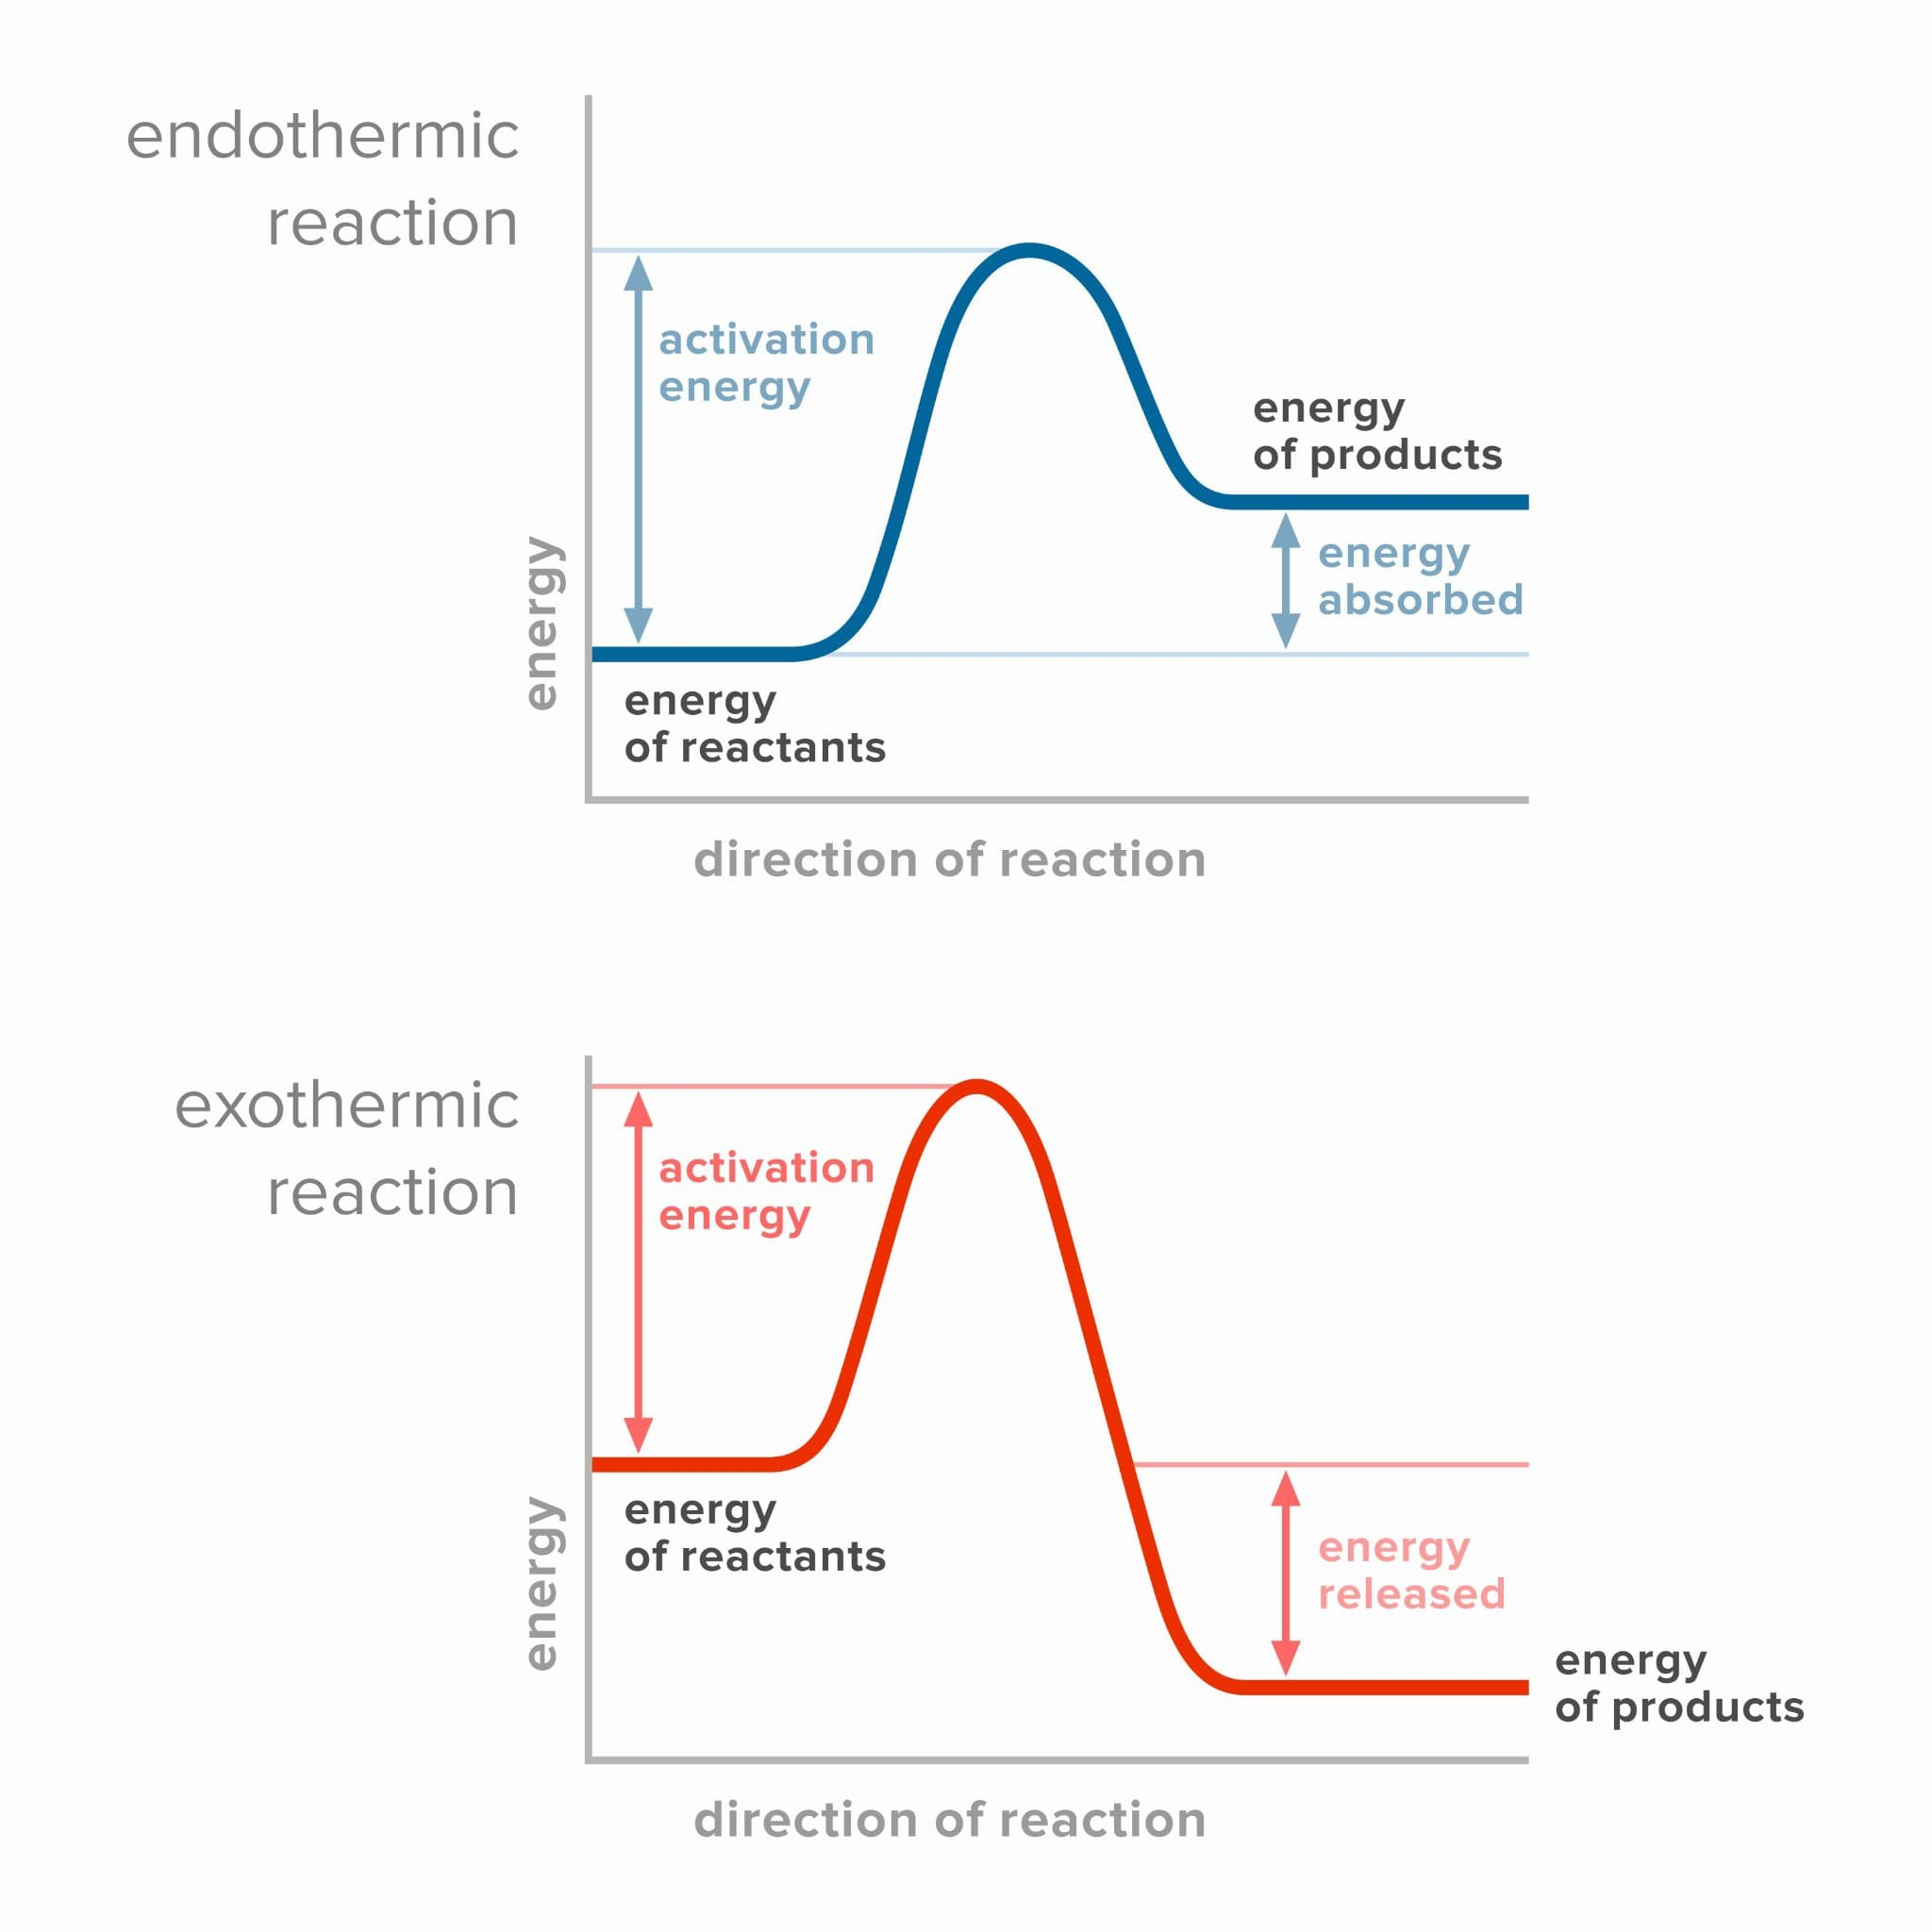
\includegraphics[width=3in]{exo_endo_diagrams.png}
\caption{}
\label{fig:exo_endo_diagrams}
\end{wrapfigure}

\index{hydrogen}Hydrogen and oxygen have a special tendency to bond with themselves. Almost 
never will you find them unbonded. Oxygen is most often found as $O_2$ and 
hydrogen as $H_2$. If you mix these together in a 2:1 ratio of hydrogen to oxygen
and light a match, they will rearrange themselves into water molecules. This is called a \textit{
chemical reaction}. In any chemical reaction, the atoms are rearranged into new
molecules.\index{chemical reaction}

When a chemical reaction happens, some bonds are
broken and new bonds are formed. The breaking and forming of bonds requires
energy. The amount of energy required to break bonds is different for different
bonds. The amount of energy released when new bonds are formed is also different
for different bonds. Some chemical reactions (like the burning of hydrogen gas described above) are
\textit{exothermic} --- that is, they give off more energy than they absorb. Burning hydrogen gas
happens quickly and gives off a lot of energy. If you have enough, it will make
quite an explosion! \index{exothermic} Other chemical reactions are \textit{endothermic} 
--- they consume energy. \index{photosynthesis}Photosynthesis, the process by which plants consume energy from the sun to make
sugar from $CO_2$ and $H_2O$ requires an endothermic chemical reaction.\index{endothermic} Energy stored in chemical bonds
is called \textit{chemical energy},\index{chemical energy} which is a form of \textit{potential energy}.

Examine the diagrams in figure \ref{fig:exo_endo_diagrams}. The $x$-axis 
represents time - time passes as we move from left to right across the diagram. 
At the far left, the energy of the \index{reactants}reactants (the ingredients that go into the 
reaction) is shown. At the far right, the energy of the \index{products}products (what is made in 
the chemical reaction) is shown. Look at the endothermic reaction diagram (the blue one). Based on the
relative energies of the reactants and products, do you expect an endothermic
reaction to release or absorb heat? Absorb! Since the products have more
energy, they must have absorbed energy, in the form of heat, from the surroundings.

Now, the red diagram shows an exothermic reaction: 
the products have less energy than the reactants. Since \index{conservation of energy}energy is never created or destroyed, where did 
the energy go? It is released as \index{heat}heat. So, exothermic reactions release heat.
What does this look and feel like in real life? If an exothermic reaction were
happening in a glass beaker, you would feel warmth if you held the beaker. The
heat is leaving the beaker and entering your hand, which feels warm. What
about an endothermic reaction? Many students think that since an endothermic
reaction absorbs heat, it must be getting hot. This is incorrect:
\textit{exothermic} reactions feel hot. If an endothermic reaction were
happening in a beaker and you touched the beaker, it would feel \textbf{cold}.
Why? Well, if the reaction is absorbing heat, then heat must be leaving it
surroundings (your hand) and entering the reaction (this heat energy is turned
into chemical energy that is stored in the new chemical bonds that are
forming). So your hand feels cold. You may have used both kinds: a hand warmer gets hot from an exothermic reaction, and an instant cold pack in a first-aid kit gets cold from an endothermic one.

\begin{Exercise}[title = {Hot or Cold?}, label = exo_endo]
For each process, say whether it is exothermic or endothermic, and whether a container holding it would feel warm or cold.
\begin{enumerate}
\item A campfire burning wood.
\item An instant cold pack, which dissolves a salt in water.
\item Plants making sugar from $CO_2$ and $H_2O$ in sunlight.
\end{enumerate}
\end{Exercise}

\begin{Answer}[ref = exo_endo]
\begin{enumerate}
\item Exothermic. It releases heat, so it feels warm (very warm!).
\item Endothermic. It absorbs heat from its surroundings, so it feels cold.
\item Endothermic. Photosynthesis stores energy from sunlight in the sugar's chemical bonds.
\end{enumerate}
\end{Answer}

%FIXME great place to talk about endergonic and exergonic reactions
